
\documentclass[11pt]{article}
\usepackage[margin=0.5in]{geometry}
\usepackage[utf8]{inputenc}
\usepackage{setspace}
\setstretch{1}
\usepackage[english]{babel}
\usepackage[]{amssymb} 
%\usepackage[enable]{darkmode} 
\usepackage{amsmath, amsthm}
\usepackage{mdframed}
\usepackage{pgfplots}
\usepackage{booktabs}
\usepackage{enumitem}
\usepackage{hyperref}
\usetikzlibrary{pgfplots.fillbetween}  
\pgfplotsset{compat=1.17} 
\makeatletter
\newcommand{\tpmod}[1]{{\@displayfalse\pmod{#1}}}
\makeatother

\mdfdefinestyle{problemstyle}{
    innertopmargin=0pt,
    innerbottommargin=10pt,
    innerrightmargin=10pt,
    innerleftmargin=10pt,
    outerlinewidth=1pt,
    topline=true,
    bottomline=true,
    leftline=true,
    rightline=true
}

%custom enviroment for exercises
\newenvironment{exercise}{
    \begin{mdframed}[style=problemstyle]\textcolor{black}{}
}{
    \end{mdframed}
}


\title{TMATH 126 Finale Review Workshop}
\author{}
\date{\vspace{-5ex}}

\begin{document}
\maketitle
\vspace{-5ex}%not a fan of this, but good fix for now

\section*{Unit 1}
Unless otherwise stated let $\vec{u} = \langle 2,-3,5 \rangle$ and 
$\vec{v} = \langle 4, -1, 2 \rangle $ 
\subsection*{1a: Coordinates and Vectors in 2D and 3D}
\begin{exercise}
    \begin{enumerate}[label={\alph*}]
        \item Draw vectors $\vec{u}$ and $\vec{v}$ in 2D and 3D. 
            Then draw $\vec{u} + \vec{v}$ using the tip-to-tail method.
        \item Draw and label $\vec{u} - \vec{v}$ on the same coordinate 
            system.
    \end{enumerate}
\end{exercise}

\subsection*{1b: Dot Product, Cross Product}
\begin{exercise}
    \begin{enumerate}[label={\alph*}]
        \item Explain the applications of the dot and cross product.
            (ie what do they tell/give us)
        \item Find the scalar projection of $\vec{u}$ onto $\vec{v}$.
        \item Find the vector projection of $\vec{v}$ onto $\vec{u}$.
        \item Find the angle between $\vec{u}$ $\vec{v}$.
        \item Find the area of a parallelogram with the points $A(0,1,3)$, 
            $B(1,3,5)$, $C(5,7,5)$, $D(4,5,3)$.
    \end{enumerate}
\end{exercise}

\subsection*{1c: Equations of Lines and Planes}
\begin{exercise}
    \begin{enumerate}[label={\alph*}]
        \item Given point $A(1,1,1)$ and $\vec{d} = \langle 10, -10, 50 \rangle$
            Write the vector equation of a line in 2D and 3D that contains point $A$ 
            moves is parallel to $\vec{d}$.
        \item Find the equation of a plane with points $(4, -3, 1)$, $(-3,-1, 1)$,
            and $4,-2, 8$.
        \item Determine if the planes given by $4x - 9y - z = 2$ and 
            $x + 2y -14z = -6$ are parallel, orthogonal, or neither.
        \item Determine where the line $\vec{r}(t) = \langle -2t, 2+7t, -1-4t \rangle$
            and the plane given by $\langle 4x + 9y - 2z = -8$ 
        \item Find the line of intersection of the planes given by 
            $3x + 6y - 5z = -3$ and $-2x + 7y - z = 24$.
        \item Find the point on the plane $3x + 4y + z = 1$ that is closest to the 
            point $(1, 0, 1)$.
    \end{enumerate}
\end{exercise}

\newpage
\subsection*{1d: Equations of Cylinders and Other Simple Surfaces}
\begin{figure}[!ht]
    \centering
    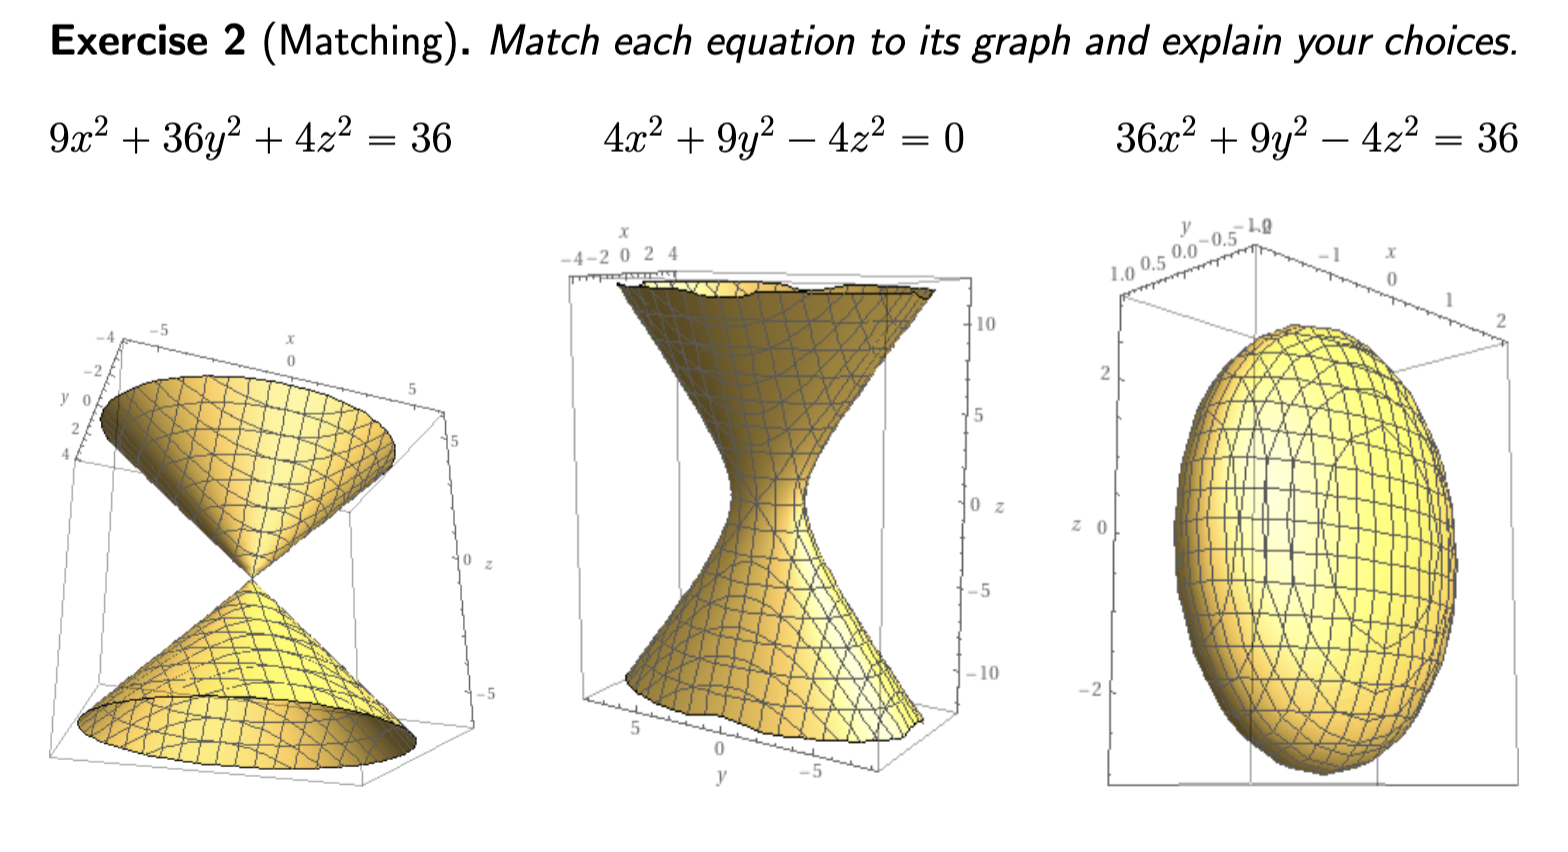
\includegraphics[width=0.5\textwidth]{images/match-practice.png}
\end{figure}
\begin{exercise}
    Identify and sketch the following 3D surfaces.
    \begin{enumerate}[label={\alph*}]
        \item $x^2 + y^2 + z^2 = 1$
        \item $x=cost$ and $y=sint$
        \item $x^2 +\frac{y^2}{9} + \frac{z^2}{4}$
        \item $z=4z^2+y^2$
    \end{enumerate}
\end{exercise}


\section*{Unit 2}
\begin{exercise}
A particle moves along a path in space described by the vector-valued function
$$\vec{r}(t) = \langle 3\cos t, 3\sin t, t^2 \rangle, \quad 0 \le t \le 2\pi.$$
\begin{enumerate}[label={\alph*}]
    \item Find the domain of $\vec{r}(t)$.

    \item Describe the motion of the particle in words. What shape does the projection of the path make in the $xy$-plane?
    
    \item Find $\vec{r}\,'(t)$ and set up an integral for the arc length of the curve from $t = 0$ to $t = 3\pi$. Then use a calculator or software to evaluate the integral.
    
    \item Find the equation of the line tangent to the curve at $t = \pi$.

    \item Let $z = f(x, y) = x^2 + y^2$. Describe the motion of the particle. Additionally what is the domain of  $\vec{r}(t)$.

\end{enumerate}
\end{exercise}

\section*{Unit 3}
\begin{exercise}
Consider the function $f(x, y) = 9 - x^2 - y^2$.
\begin{enumerate}[label={\alph*}]
    \item Sketch at least three level curves of $f(x, y)$ for the values $f(x, y) = 0$, $4$, and $8$. Label each curve clearly.
    
    \item Describe the shape of the surface $z = f(x, y)$. What kind of surface is it? What do the level curves represent geometrically?
\end{enumerate}
\end{exercise}

\newpage
\begin{exercise}
Consider the function $$f(x, y) = x^3 - 3xy^2.$$

\begin{enumerate}[label={\alph*}]

\item  
Compute the first-order partial derivatives $f_x(x, y)$ and $f_y(x, y)$. 

\item Find the equation of the tangent plane to the surface at point $P = (1,1, f(1,1))$.  
    Write the linear approximation of $f(x,y)$ near $P$.  

\item 
Calculate the gradient vector $\nabla f(1,1)$.  
Find the directional derivative of $f$ at point $P$ in the direction of the vector $\mathbf{v} = \langle 2, 1 \rangle$ .  
Determine the direction of fastest increase of $f$ at $P$.

\item 
    Use the result from part (c) to write the equation of the line tangent to the surface 
    $f(x, y)$ at the point $P = (1,1, f(1,1))$ in the direction of the vector $\mathbf{v} = \langle 2, 1 \rangle$.  

\item  
    Find all critical points of $f(x,y)$ and classify them(local extrema, saddle points, etc). 
    Use the second derivative test (Hessian matrix).

\end{enumerate}
\end{exercise}

\begin{exercise}
\begin{enumerate}[label={\alph*}]
    \item 
        consider the integral $\iint_D sin(y^2)\, dA$ where $D$ is the region
        bounded by $y=x$ and the $y-axis$ from $x=0$ to $x=1$
        (set up and solve the integral both ways, one of these integrals will not be possible)
    \item $\iint_D e^{\frac{x}{y}}\, dA$, Where $D$ is bounded by $y=\sqrt{x}$ and $y=x^3$ 
\end{enumerate}
\end{exercise}

\begin{exercise}
    \begin{enumerate}[label={\alph*}]
        \item let $f(x) = \frac{16}{4-x^2} + 6cos(x)$
        \item Give the Taylor series for $f$ based at $b=0$ using one sigma
        sine.
        \item Find the largest open interval on which this taylor series converges.
        \item Find $T_3(x)$, the third Taylor polynomial for $f$ based at $b=0$. Then 
        estimate the value of $\int_0^1 f(x)dx$ by replacing $f(x)$ with $T_3(x)$.
    \end{enumerate}
\end{exercise}
\end{document}

